\documentclass{standalone}
\usepackage{tikz}

\begin{document}

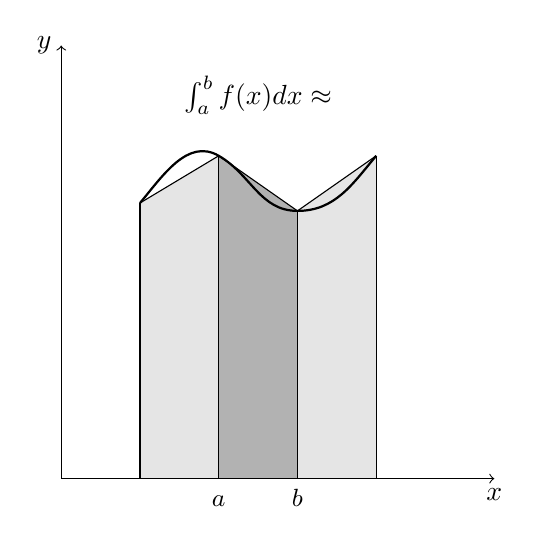
\begin{tikzpicture}
\coordinate (p1) at (0.7,3);
\coordinate (p2) at (1,3.3);
\coordinate (p3) at (2,2.5);
\coordinate (p4) at (3,2.5);
\coordinate (p5) at (4,3.5);
\coordinate (p6) at (5,4.1);
\coordinate (p7) at (6,3.4);
\coordinate (p8) at (7,4.1);
\coordinate (p9) at (8,4.6);
\coordinate (p10) at (9,4);
\coordinate (p11) at (9.5,4.7);

% The cyan background
\fill[gray!20] 
  (p5|-0,0) -- (p5) -- (p6) -- (p7) -- (p8) -- (p8|-0,0) -- cycle;
% the dark cyan stripe
\fill[gray!60] (p6|-0,0) -- (p6) -- (p7) -- (p7|-0,0) -- cycle;
% the curve
\draw[thick,black] 
  (p5) to[out=50,in=150] (p6) to[out=-30,in=180] 
  (p7) to[out=0,in=230] (p8);
% the broken line connecting points on the curve
\draw (p5) -- (p6) -- (p7) -- (p8);
% vertical lines and labels
\foreach \n/\texto in {5/{},6/{a},7/{b},8/{}}
{
  \draw (p\n|-0,0) -- (p\n);
  \node[below,text height=1.5ex,text depth=1ex,font=\small] at (p\n|-0,0) {$\texto$};
}
% The axes
\draw[->] (3,0) -- (8.5,0) coordinate (x axis);
\draw[->] (3,0) -- (3,5.5) coordinate (y axis);
% labels for the axes
\node[below] at (x axis) {$x$};
\node[left] at (y axis) {$y$};
% label for the function
\node[above,text=black] at (5.5,4.5) {$\int_a^b f(x) dx \approx$};
\end{tikzpicture}

\end{document}

% This is modified from the following source:
% http://tex.stackexchange.com/questions/110598/trapezium-rule-for-integration-using-tikz